\documentclass[border=2pt]{standalone}
\usepackage{amsmath}
\usepackage{tikz}
\usetikzlibrary{decorations.pathreplacing}
\begin{document}
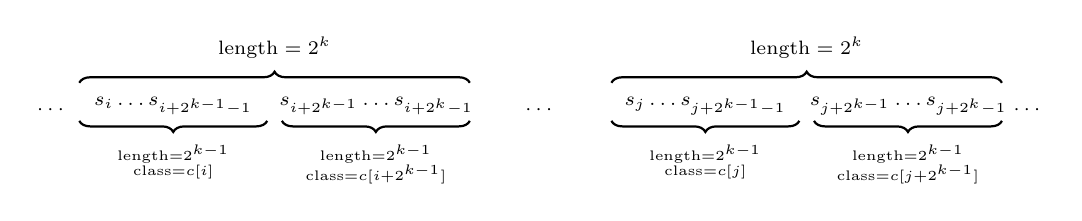
\begin{tikzpicture}[x=0.62cm,y=0.62cm, every node/.style={font=\scriptsize}]
  \node at (-0.55,-0.55) {$\cdots$};

  \draw[thick,decorate,decoration={brace,amplitude=4pt}] (0,0) -- (8,0)
    node[midway,above=5pt] {$\mathrm{length}=2^k$};
  \draw[thick,decorate,decoration={brace,mirror,amplitude=4pt}] (0,-0.78) -- (3.85,-0.78)
    node[midway,below=5pt] {$\substack{\mathrm{length}=2^{k-1}\\\mathrm{class}=c[i]}$};
  \draw[thick,decorate,decoration={brace,mirror,amplitude=4pt}] (4.15,-0.78) -- (8,-0.78)
    node[midway,below=5pt] {$\substack{\mathrm{length}=2^{k-1}\\\mathrm{class}=c[i+2^{k-1}]}$};
  \node at (1.92,-0.48) {$s_i\ldots s_{i+2^{k-1}-1}$};
  \node at (6.08,-0.48) {$s_{i+2^{k-1}}\ldots s_{i+2^k-1}$};

  \node at (9.45,-0.55) {$\cdots$};

  \draw[thick,decorate,decoration={brace,amplitude=4pt}] (10.9,0) -- (18.9,0)
    node[midway,above=5pt] {$\mathrm{length}=2^k$};
  \draw[thick,decorate,decoration={brace,mirror,amplitude=4pt}] (10.9,-0.78) -- (14.75,-0.78)
    node[midway,below=5pt] {$\substack{\mathrm{length}=2^{k-1}\\\mathrm{class}=c[j]}$};
  \draw[thick,decorate,decoration={brace,mirror,amplitude=4pt}] (15.05,-0.78) -- (18.9,-0.78)
    node[midway,below=5pt] {$\substack{\mathrm{length}=2^{k-1}\\\mathrm{class}=c[j+2^{k-1}]}$};
  \node at (12.82,-0.48) {$s_j\ldots s_{j+2^{k-1}-1}$};
  \node at (16.98,-0.48) {$s_{j+2^{k-1}}\ldots s_{j+2^k-1}$};

  \node at (19.45,-0.55) {$\cdots$};
\end{tikzpicture}
\end{document}
